\documentclass{tufte-handout}

\usepackage{graphicx} % allow embedded images
  \setkeys{Gin}{width=\linewidth,totalheight=\textheight,keepaspectratio}
  \graphicspath{{graphics/}} % set of paths to search for images
\usepackage{amsmath}  % extended mathematics
\usepackage{fancyvrb} % extended verbatim environments
  \fvset{fontsize=\normalsize}% default font size for fancy-verbatim environments
\usepackage{minted}
\usemintedstyle{xcode}
\usepackage{listings}
\usepackage{enumitem}
\usepackage{tikz}
% Standardize command font styles and environments
\newcommand{\doccmd}[1]{\texttt{\textbackslash#1}}% command name -- adds backslash automatically
\newcommand{\docopt}[1]{\ensuremath{\langle}\textrm{\textit{#1}}\ensuremath{\rangle}}% optional command argument
\newcommand{\docarg}[1]{\textrm{\textit{#1}}}% (required) command argument
\newcommand{\docenv}[1]{\textsf{#1}}% environment name
\newcommand{\docpkg}[1]{\texttt{#1}}% package name
\newcommand{\doccls}[1]{\texttt{#1}}% document class name
\newcommand{\docclsopt}[1]{\texttt{#1}}% document class option name
\newenvironment{docspec}{\begin{quote}\noindent}{\end{quote}}% command specification environment


\lstnewenvironment{sexp}{\lstset{basicstyle=\ttfamily,language=Lisp}}{}
\lstnewenvironment{mexp}{\lstset{basicstyle=\ttfamily,mathescape}}{}
\newcommand{\macroequiv}[0]{\overset{\mathtt{MACRO}}{\mathbf{\equiv}}}
\newcommand{\alphabeta}[0]{$\alpha$-$\beta$~}

\title{The \alphabeta Heuristic}
\author[Edwards, D.J, Timothy P. Hart]{Edwards, D.J, Timothy P. Hart}
\date{October 28, 1963} % without \date command, current date is supplied

\newtheorem{theorem}{Theorem}
\begin{document}

\maketitle% this prints the handout title, author, and date

The \alphabeta heuristic is a method for pruning unneeded branches from the move
tree of a game. The algorithm makes use of information gained about part of the
tree to reject those branches which will not affect the principle variation.

The reasoning behind the \alphabeta heuristic is as follows:
\begin{enumerate}[label=\alph*)]
\item if the maximizing-player finds a move whose value is greater than or equal
  to the value of an alternate minimising-player move found higher in the tree,
  he should not look further because the min-player would certainly take that
  alternate move.
\item if the min-player finds a move whose value is less than or equal to the
  value of an alternate max-player move found higher in the tree, he should not
  look further because the max-player would certainly thake that alternate move.
\end{enumerate}

\begin{center}
  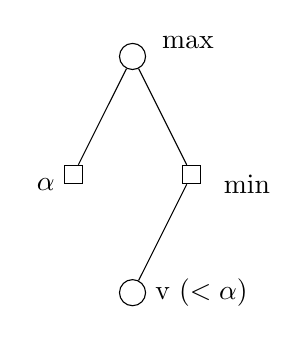
\begin{tikzpicture}
    \node[circle, draw] (max) {}
    child { node [rectangle, draw] (alpha) {}}
    child { node[rectangle, draw] (min) {}
      child { node [circle, draw] (vee) {}}
      child[missing] { node [] {}}};
    
    \node[xshift=2em] at (max.north) {max};
    \node[xshift=-1em] at (alpha.south) {$\alpha$};
    \node[xshift=2em] at (min.south) {min};
    \node[xshift=2em] at (vee.east) {v ($< \alpha$)};
  \end{tikzpicture}
\end{center}

Case (b) may be illustrated by the above piece of tree. The max-player has
investigated the branch with value $\alpha$ and has looked at an alternate move
from the point at which this branch was found. At the time the value v is
established the maximizing player (whose point of view we are taking) sees that
if he takes the right branch from the top node he is giving the other player the
opportunity to take the v branch. But this will result in his getting v or less,
and since he can get $\alpha$ by taking the left branch, he instantly decides he
won't make the move to the right under any circumstance.

The following definitions express the \alphabeta heuristic:

\begin{mexp}
  vmax[pos;$\alpha$;$\beta$] = [if final[pos;$\alpha$;$\beta$] then evaluate [pos]
                   else vlmax[succ[pos];$\alpha$;$\beta$]]
  vlmax[lis;$\alpha$;$\beta$] = [if null[lis] then $\alpha$
                   else if vmin[car[lis];$\alpha$;$\beta$] $\geq \beta$ then $\beta$
                   else vlmax[cdr[lis];
                              max[vmin[car[lis];$\alpha$;$\beta$]$\alpha$];
                              $\beta$]]
  vmin[pos;$\alpha$;$\beta$] = [if final[pos;$\alpha$;$\beta$] then evaluate[pos]                                
                   else vlmin[succ[pos];$\alpha$;$\beta$]]
  vlmin[lis;$\alpha$;$\beta$] = [if null[lis] then $\beta$
                   else if vmax[car[lis];$\alpha$;$\beta$] $\leq \alpha$ then $\alpha$
                   else vlmin[cdr[lis];
                              $\alpha$;
                              min[vmax[car[lis];$\alpha$;$\beta$];$\beta$]]]
\end{mexp}
where:
\begin{itemize}
\item[] \texttt{pos} stands for some representation of the current position.
\item[] \texttt{lis} is a list of position representatoins.
\item[] \texttt{succ[pos]} is a function which produces a list of positions
  which can be reached in one move from \texttt{pos}.
\item[] \texttt{final[pos;$\alpha$;$\beta$]} is a predicate which may decide
  that the search is not to continue, e.g., when the end of the game has been
  reached.
\item[] \texttt{evaluate[pos]} provides some measure of goodness of the position
  (always from the point of view of maximising player).
\item[] $\alpha$ and $\beta$ are initially set at $-\infty$ and $+\infty$ respectively.
\end{itemize}

This heuristic may readily be compared with a minimax search by observing that
if the second clauses in the conditional expression \texttt{vlmax} and
\texttt{vlmin} are eliminated the resulting function is just minimax.

It is important to note that the ordering of the list of moves generated by
\texttt{succ} is very important. The most gain is achieved from the heuristic
when the right move is at the beginning of the list.

It turns out that the best, that is, in the case of perfect ordering the
\alphabeta heuristic can cut a tree's exponential growth rate in half, thus
allowing almost twice the search depth for the same effort. More precisely, we
have the following theorem.

\begin{theorem}[Levin]
  Let $n$ be the number of plies in a tree, and let $b$ be the number of
  branches at every branch point. Then the number of terminal points on the tree is
  $$T = b^n$$

  However, if the best possible advantage is taken of the \alphabeta heristic
  then the number of terminal point that need be examined is
  \begin{eqnarray*}
    T =& b^{\frac{n+1}{2}} + b^{\frac{n-1}{2}} &\text{for odd}~n\\
    T =& 2b^{\frac{n}{2}} - 1 &\text{for even}~n
  \end{eqnarray*}  
\end{theorem}

Example: %TODO

\begin{center}
  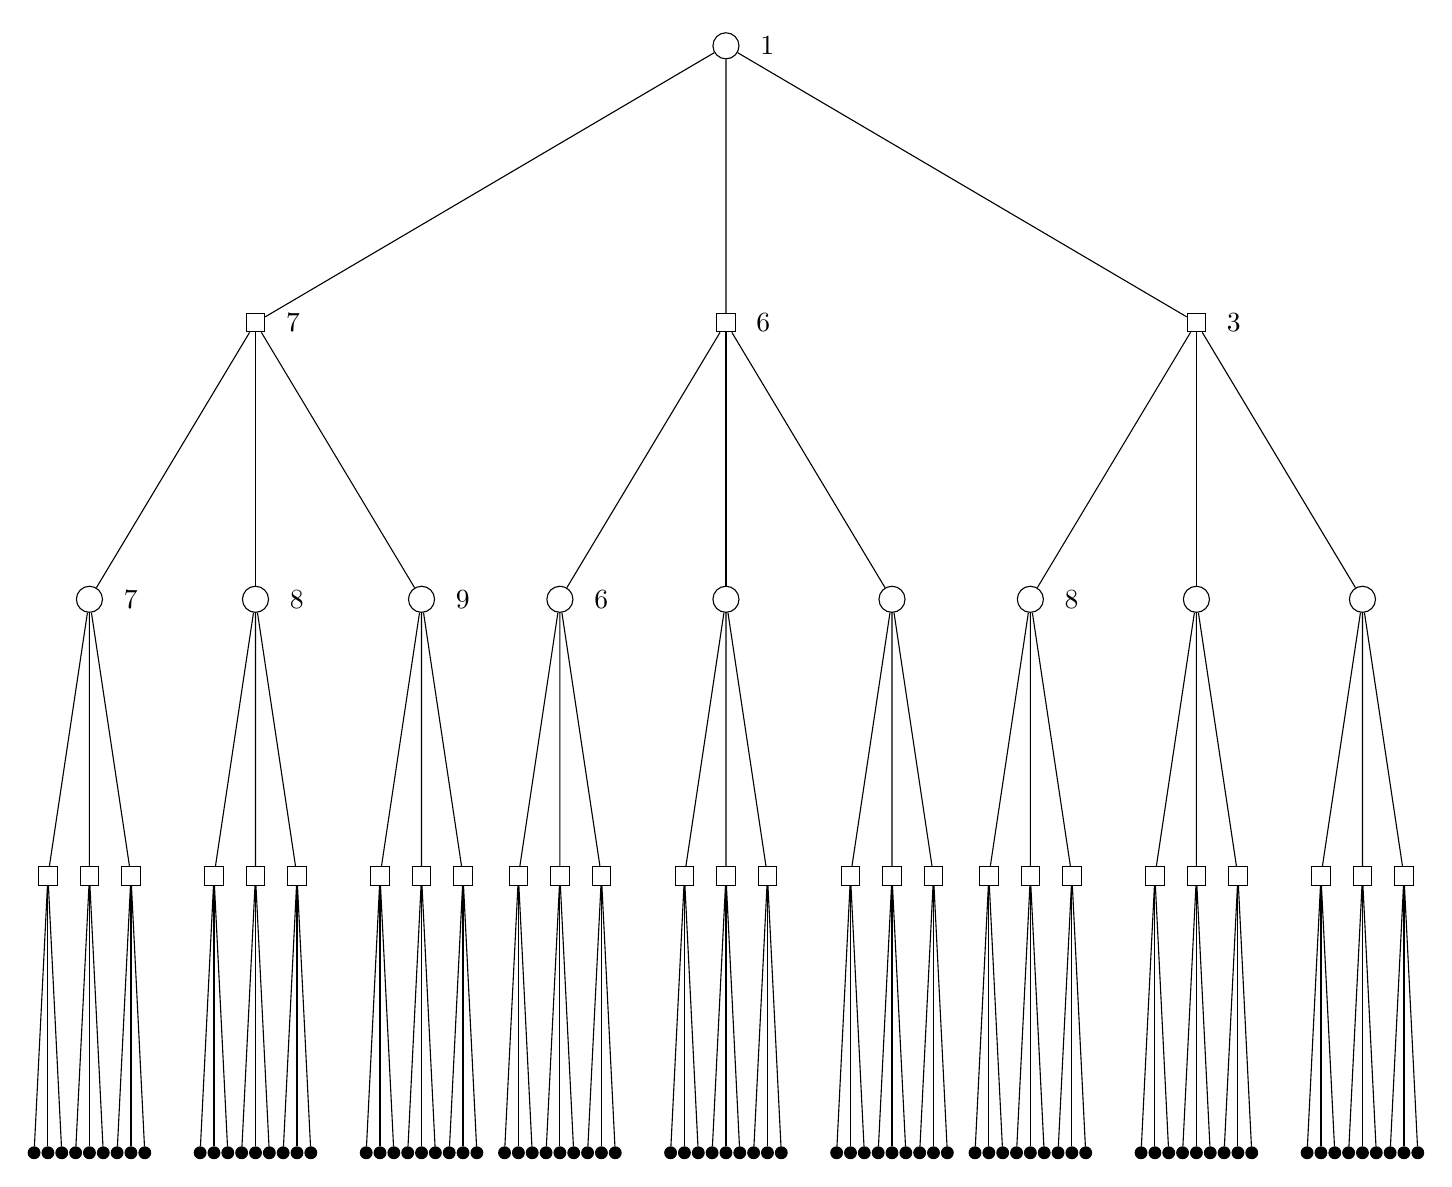
\begin{tikzpicture}
    \tikzset{
      level/.style = {level distance=10em},
      level 1/.style = {sibling distance=17em},
      level 2/.style = {sibling distance=6em},
      level 3/.style = {sibling distance=1.5em},
      level 4/.style = {sibling distance=.5em}
      }
    \tikzstyle{maximizing}=[circle, draw]
    \tikzstyle{minimizing}=[rectangle, draw]
    \tikzstyle{terminal}=[circle, draw, inner sep=1.5, fill=black]
    \tikzstyle{right-label}=[xshift=1em]

    \node[maximizing] (root) {}

    % (loop for i from 1 to 3
    % do (format t "child {node[minimizing] (g1~a) {}~%" i)
    %   (loop for j from 1 to 3
    %   do (format t "    child {node[maximizing] (g2~a~a) {}~%" i j)
    %     (loop for k from 1 to 3
    %     do (format t "        child {node[minimizing] (g3~a~a) {}~%" j k)
    %       (loop for l from 1 to 3
    %       do (format t "            child {node[terminal] (g4~a~a) {}}~%" k l))
    %       (format t "        }~%"))
    %     (format t "    }~%"))
    %   (format t "}~%"))
    child {node[minimizing] (g11) {}
      child {node[maximizing] (g211) {}
        child {node[minimizing] (g311) {}
          child {node[terminal] (g411) {}}
          child {node[terminal] (g412) {}}
          child {node[terminal] (g413) {}}
        }
        child {node[minimizing] (g312) {}
          child {node[terminal] (g421) {}}
          child {node[terminal] (g422) {}}
          child {node[terminal] (g423) {}}
        }
        child {node[minimizing] (g313) {}
          child {node[terminal] (g431) {}}
          child {node[terminal] (g432) {}}
          child {node[terminal] (g433) {}}
        }
      }
      child {node[maximizing] (g212) {}
        child {node[minimizing] (g321) {}
          child {node[terminal] (g411) {}}
          child {node[terminal] (g412) {}}
          child {node[terminal] (g413) {}}
        }
        child {node[minimizing] (g322) {}
          child {node[terminal] (g421) {}}
          child {node[terminal] (g422) {}}
          child {node[terminal] (g423) {}}
        }
        child {node[minimizing] (g323) {}
          child {node[terminal] (g431) {}}
          child {node[terminal] (g432) {}}
          child {node[terminal] (g433) {}}
        }
      }
      child {node[maximizing] (g213) {}
        child {node[minimizing] (g331) {}
          child {node[terminal] (g411) {}}
          child {node[terminal] (g412) {}}
          child {node[terminal] (g413) {}}
        }
        child {node[minimizing] (g332) {}
          child {node[terminal] (g421) {}}
          child {node[terminal] (g422) {}}
          child {node[terminal] (g423) {}}
        }
        child {node[minimizing] (g333) {}
          child {node[terminal] (g431) {}}
          child {node[terminal] (g432) {}}
          child {node[terminal] (g433) {}}
        }
      }
    }
    child {node[minimizing] (g12) {}
      child {node[maximizing] (g221) {}
        child {node[minimizing] (g311) {}
          child {node[terminal] (g411) {}}
          child {node[terminal] (g412) {}}
          child {node[terminal] (g413) {}}
        }
        child {node[minimizing] (g312) {}
          child {node[terminal] (g421) {}}
          child {node[terminal] (g422) {}}
          child {node[terminal] (g423) {}}
        }
        child {node[minimizing] (g313) {}
          child {node[terminal] (g431) {}}
          child {node[terminal] (g432) {}}
          child {node[terminal] (g433) {}}
        }
      }
      child {node[maximizing] (g222) {}
        child {node[minimizing] (g321) {}
          child {node[terminal] (g411) {}}
          child {node[terminal] (g412) {}}
          child {node[terminal] (g413) {}}
        }
        child {node[minimizing] (g322) {}
          child {node[terminal] (g421) {}}
          child {node[terminal] (g422) {}}
          child {node[terminal] (g423) {}}
        }
        child {node[minimizing] (g323) {}
          child {node[terminal] (g431) {}}
          child {node[terminal] (g432) {}}
          child {node[terminal] (g433) {}}
        }
      }
      child {node[maximizing] (g223) {}
        child {node[minimizing] (g331) {}
          child {node[terminal] (g411) {}}
          child {node[terminal] (g412) {}}
          child {node[terminal] (g413) {}}
        }
        child {node[minimizing] (g332) {}
          child {node[terminal] (g421) {}}
          child {node[terminal] (g422) {}}
          child {node[terminal] (g423) {}}
        }
        child {node[minimizing] (g333) {}
          child {node[terminal] (g431) {}}
          child {node[terminal] (g432) {}}
          child {node[terminal] (g433) {}}
        }
      }
    }
    child {node[minimizing] (g13) {}
      child {node[maximizing] (g231) {}
        child {node[minimizing] (g311) {}
          child {node[terminal] (g411) {}}
          child {node[terminal] (g412) {}}
          child {node[terminal] (g413) {}}
        }
        child {node[minimizing] (g312) {}
          child {node[terminal] (g421) {}}
          child {node[terminal] (g422) {}}
          child {node[terminal] (g423) {}}
        }
        child {node[minimizing] (g313) {}
          child {node[terminal] (g431) {}}
          child {node[terminal] (g432) {}}
          child {node[terminal] (g433) {}}
        }
      }
      child {node[maximizing] (g232) {}
        child {node[minimizing] (g321) {}
          child {node[terminal] (g411) {}}
          child {node[terminal] (g412) {}}
          child {node[terminal] (g413) {}}
        }
        child {node[minimizing] (g322) {}
          child {node[terminal] (g421) {}}
          child {node[terminal] (g422) {}}
          child {node[terminal] (g423) {}}
        }
        child {node[minimizing] (g323) {}
          child {node[terminal] (g431) {}}
          child {node[terminal] (g432) {}}
          child {node[terminal] (g433) {}}
        }
      }
      child {node[maximizing] (g233) {}
        child {node[minimizing] (g331) {}
          child {node[terminal] (g411) {}}
          child {node[terminal] (g412) {}}
          child {node[terminal] (g413) {}}
        }
        child {node[minimizing] (g332) {}
          child {node[terminal] (g421) {}}
          child {node[terminal] (g422) {}}
          child {node[terminal] (g423) {}}
        }
        child {node[minimizing] (g333) {}
          child {node[terminal] (g431) {}}
          child {node[terminal] (g432) {}}
          child {node[terminal] (g433) {}}
        }
      }
    };    

    \node[right-label] at (root.east) {$1$};

    \node[right-label] at (g11.east) {$7$};
    \node[right-label] at (g12.east) {$6$};
    \node[right-label] at (g13.east) {$3$};

    \node[right-label] at (g211.east) {$7$};
    \node[right-label] at (g212.east) {$8$};
    \node[right-label] at (g213.east) {$9$};
    \node[right-label] at (g221.east) {$6$};
    \node[right-label] at (g231.east) {$8$};
    

\end{tikzpicture}
\end{center}


This example shows an ordered ternary tree where only the labelled terminal
nodes need be examined. According to the formula for $n$ even where $b = 3$ and
$n = 4$ only $17$ out of the $81$ possible nodes need to be examined and this is
shown to be true in this case. Note that the unlabelled n odes may have any
possible value and the result will still be unchanged.

\end{document}

%%% Local Variables:
%%% mode: latex
%%% TeX-command-extra-options: "-shell-escape"
%%% TeX-master: "aim-030"
%%% End:
